\chapter{Export}
\begin{figure}[!hbp]
	\centering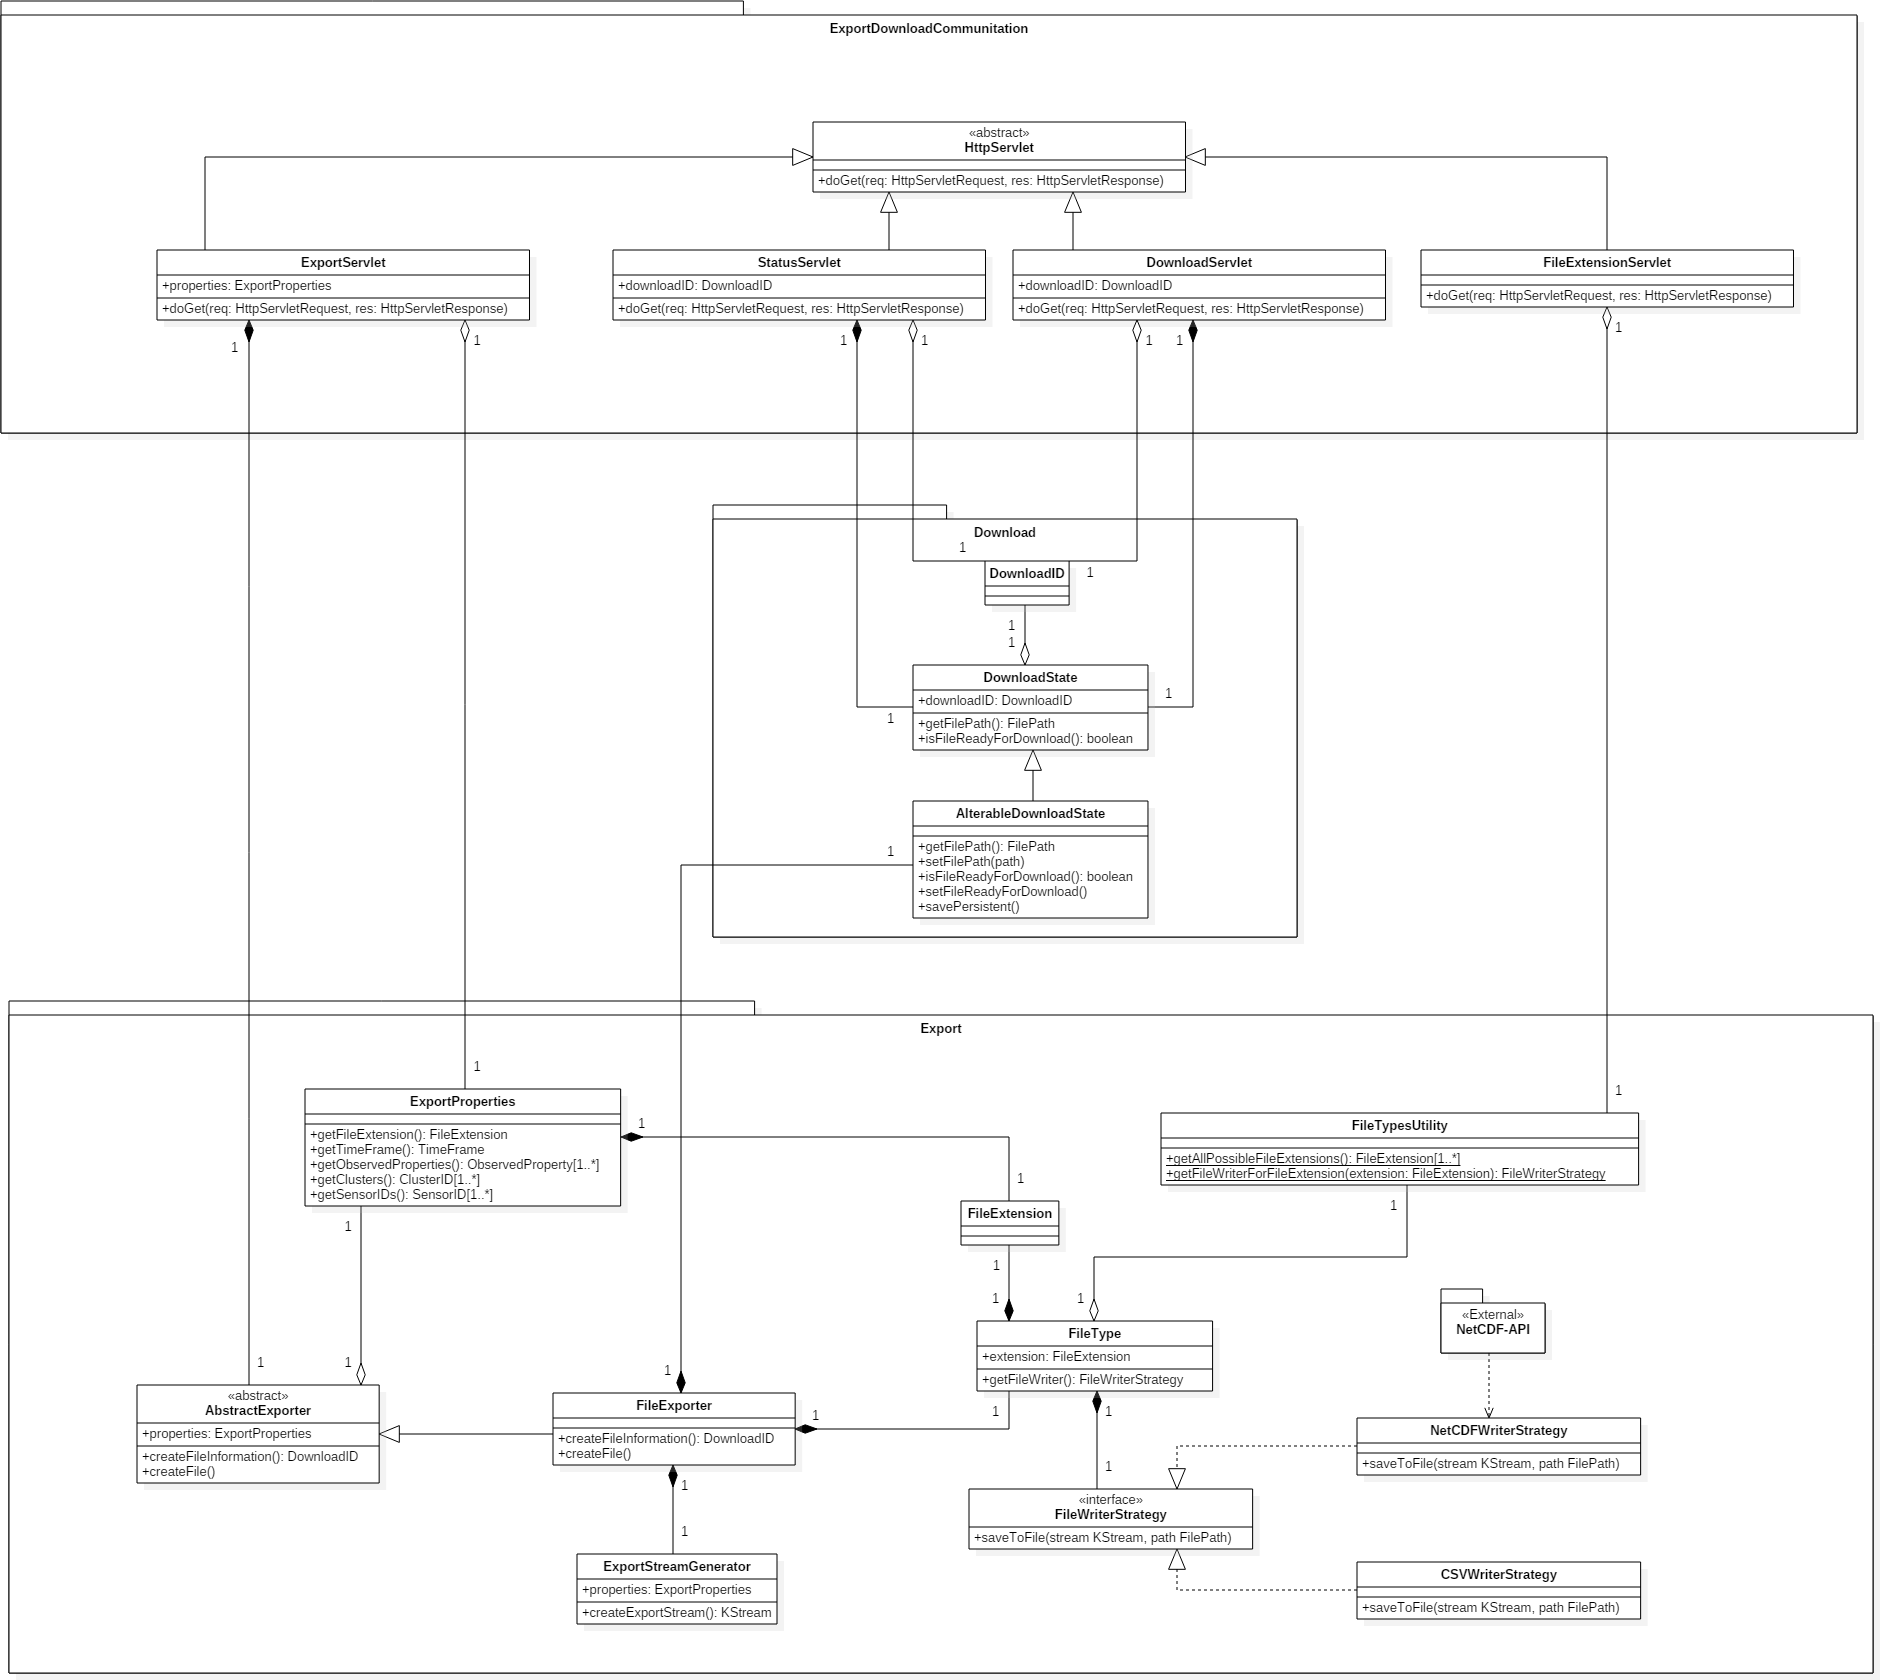
\includegraphics[width=\linewidth]{images/export/PackagedExportClassDiagram.png}
	\caption{Klassendiagramm Export und Download}
\end{figure}
\section{Package Export}{
\label{Export}\hypertarget{Export}{}
\hskip -.05in
\hbox to \hsize{\textit{ Package Contents\hfil Page}}
\vskip .13in
\hbox{{\bf  Interfaces}}
\entityintro{FileWriterStrategy}{Export.FileWriterStrategy}{Interface for the FileWriterStrategy classes.}
\vskip .13in
\hbox{{\bf  Classes}}
\entityintro{AbstractExporter}{Export.AbstractExporter}{Abstract Exporter of Data to a File.}
\entityintro{CSVWriterStrategy}{Export.CSVWriterStrategy}{Implementation of the FileWriterStrategy interface for CSV files.}
\entityintro{ExportProperties}{Export.ExportProperties}{Contains the Properties of an Export Request.}
\entityintro{ExportStreamGenerator}{Export.ExportStreamGenerator}{Generates a Stream for the Export by asking for one at the PaVoS Core and Subscribing to it.}
\entityintro{FileExporter}{Export.FileExporter}{Exporter of Data from Kafka to a File.}
\entityintro{FileExtension}{Export.FileExtension}{Represents the FileExtension of a File.}
\entityintro{FileType}{Export.FileType}{Is used to store a FileExtension information and give the right FileWriter for this FileExtension.}
\entityintro{FileTypesUtility}{Export.FileTypesUtility}{Utility class that provides static methods to get all supported FileExtensions and one to get a new Instance of the FileWriter associated with a given FileExtension.}
\entityintro{NetCDFWriterStrategy}{Export.NetCDFWriterStrategy}{Implementation of the FileWriterStrategy interface for NetCDF files.}
\vskip .1in
\vskip .1in
\newpage
\subsection{\label{Export.FileWriterStrategy}Interface FileWriterStrategy}{
\hypertarget{Export.FileWriterStrategy}{}\vskip .1in
Interface for the FileWriterStrategy classes. Realization of a Strategy to be able to swap out the way a File has to be saved.\vskip .1in
\begin{figure}[!hbp]
	\centering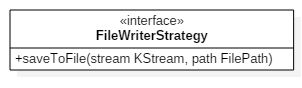
\includegraphics[width=0.5\linewidth]{images/export/classes/FileWriterStrategy}
\end{figure}
\subsubsection{Declaration}{
\begin{lstlisting}[frame=none]
public interface FileWriterStrategy
\end{lstlisting}
\subsubsection{All known subinterfaces}{NetCDFWriterStrategy\small{\refdefined{Export.NetCDFWriterStrategy}}, CSVWriterStrategy\small{\refdefined{Export.CSVWriterStrategy}}}
\subsubsection{All classes known to implement interface}{NetCDFWriterStrategy\small{\refdefined{Export.NetCDFWriterStrategy}}, CSVWriterStrategy\small{\refdefined{Export.CSVWriterStrategy}}}
\subsubsection{Method summary}{
\begin{verse}
\hyperlink{Export.FileWriterStrategy.saveToFile(KStream, FilePath)}{{\bf saveToFile(KStream, FilePath)}} Creates a File as specified by the FilePath and saves the Data from the provided KafkaStream into it.\\
\end{verse}
}
\subsubsection{Methods}{
\vskip -2em
\begin{itemize}
\item{
\index{saveToFile(KStream, FilePath)}
\hypertarget{Export.FileWriterStrategy.saveToFile(KStream, FilePath)}{{\bf  saveToFile}\\}
\begin{lstlisting}[frame=none]
void saveToFile(KStream stream,FilePath path)\end{lstlisting} %end signature
\begin{itemize}
\item{
{\bf  Description}

Creates a File as specified by the FilePath and saves the Data from the provided KafkaStream into it.
}
\item{
{\bf  Parameters}
  \begin{itemize}
   \item{
\texttt{stream} -- is the KStream, that should be exported to a File.}
   \item{
\texttt{path} -- Is the FilePath, where the new File should be created.}
  \end{itemize}
}%end item
\end{itemize}
}%end item
\end{itemize}
}
}
\subsection{\label{Export.AbstractExporter}Class AbstractExporter}{
\hypertarget{Export.AbstractExporter}{}\vskip .1in
Abstract Exporter of Data to a File.\vskip .1in
\begin{figure}[!hbp]
	\centering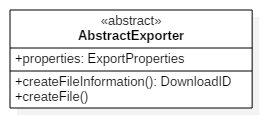
\includegraphics[width=0.4\linewidth]{images/export/classes/AbstractExporter}
\end{figure}
\subsubsection{Declaration}{
\begin{lstlisting}[frame=none]
public class AbstractExporter
 extends java.lang.Object\end{lstlisting}
\subsubsection{All known subclasses}{FileExporter\small{\refdefined{Export.FileExporter}}}
\subsubsection{Field summary}{
\begin{verse}
\hyperlink{Export.AbstractExporter.properties}{{\bf properties}} Contains the Properties of an Export Request.\\
\end{verse}
}
\subsubsection{Constructor summary}{
\begin{verse}
\hyperlink{Export.AbstractExporter()}{{\bf AbstractExporter()}} Default constructor\\
\end{verse}
}
\subsubsection{Method summary}{
\begin{verse}
\hyperlink{Export.AbstractExporter.createFile()}{{\bf createFile()}} Generates the File with the desired Data.\\
\hyperlink{Export.AbstractExporter.createFileInformation()}{{\bf createFileInformation()}} Creates Information for that Export.\\
\end{verse}
}
\subsubsection{Fields}{
\begin{itemize}
\item{
\index{properties}
\label{Export.AbstractExporter.properties}\hypertarget{Export.AbstractExporter.properties}{\texttt{public ExportProperties\ {\bf  properties}}
}
\begin{itemize}
\item{\vskip -.9ex
Contains the Properties of an Export Request.}
\end{itemize}
}
\end{itemize}
}
\subsubsection{Constructors}{
\vskip -2em
\begin{itemize}
\item{
\index{AbstractExporter()}
\hypertarget{Export.AbstractExporter()}{{\bf  AbstractExporter}\\}
\begin{lstlisting}[frame=none]
public AbstractExporter()\end{lstlisting} %end signature
\begin{itemize}
\item{
{\bf  Description}

Default constructor
}
\end{itemize}
}%end item
\end{itemize}
}
\subsubsection{Methods}{
\vskip -2em
\begin{itemize}
\item{
\index{createFile()}
\hypertarget{Export.AbstractExporter.createFile()}{{\bf  createFile}\\}
\begin{lstlisting}[frame=none]
public void createFile()\end{lstlisting} %end signature
\begin{itemize}
\item{
{\bf  Description}

Generates the File with the desired Data.
}
\end{itemize}
}%end item
\item{
\index{createFileInformation()}
\hypertarget{Export.AbstractExporter.createFileInformation()}{{\bf  createFileInformation}\\}
\begin{lstlisting}[frame=none]
public DownloadID createFileInformation()\end{lstlisting} %end signature
\begin{itemize}
\item{
{\bf  Description}

Creates Information for that Export. These Information will be used to identifie a File for the WebGUI, that gets the created DownloadID.
}
\item{{\bf  Returns} --
Is the DownloadID for the started Export.
}%end item
\end{itemize}
}%end item
\end{itemize}
}
}
\subsection{\label{Export.CSVWriterStrategy}Class CSVWriterStrategy}{
\hypertarget{Export.CSVWriterStrategy}{}\vskip .1in
Implementation of the FileWriterStrategy interface for CSV files.\vskip .1in
\begin{figure}[!hbp]
	\centering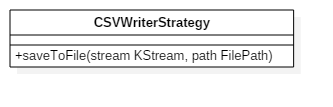
\includegraphics[width=0.5\linewidth]{images/export/classes/CSVWriterStrategy}
\end{figure}
\subsubsection{Declaration}{
\begin{lstlisting}[frame=none]
public class CSVWriterStrategy
 extends java.lang.Object implements FileWriterStrategy\end{lstlisting}
\subsubsection{Constructor summary}{
\begin{verse}
\hyperlink{Export.CSVWriterStrategy()}{{\bf CSVWriterStrategy()}} Default constructor\\
\end{verse}
}
\subsubsection{Method summary}{
\begin{verse}
\hyperlink{Export.CSVWriterStrategy.saveToFile(KStream, FilePath)}{{\bf saveToFile(KStream, FilePath)}} Creates a File as specified by the FilePath and saves the Data from the provided KafkaStream into it.\\
\hyperlink{Export.CSVWriterStrategy.saveToFile(KStream, FilePath)}{{\bf saveToFile(KStream, FilePath)}} Creates a File as specified by the FilePath and saves the Data from the provided KafkaStream into it.\\
\end{verse}
}
\subsubsection{Constructors}{
\vskip -2em
\begin{itemize}
\item{
\index{CSVWriterStrategy()}
\hypertarget{Export.CSVWriterStrategy()}{{\bf  CSVWriterStrategy}\\}
\begin{lstlisting}[frame=none]
public CSVWriterStrategy()\end{lstlisting} %end signature
\begin{itemize}
\item{
{\bf  Description}

Default constructor
}
\end{itemize}
}%end item
\end{itemize}
}
\subsubsection{Methods}{
\vskip -2em
\begin{itemize}
\item{
\index{saveToFile(KStream, FilePath)}
\hypertarget{Export.CSVWriterStrategy.saveToFile(KStream, FilePath)}{{\bf  saveToFile}\\}
\begin{lstlisting}[frame=none]
public void saveToFile(KStream stream,FilePath path)\end{lstlisting} %end signature
\begin{itemize}
\item{
{\bf  Description}

Creates a File as specified by the FilePath and saves the Data from the provided KafkaStream into it.
}
\item{
{\bf  Parameters}
  \begin{itemize}
   \item{
\texttt{stream} -- is the KStream, that should be exported to a File.}
   \item{
\texttt{path} -- Is the FilePath, where the new File should be created.}
  \end{itemize}
}%end item
\end{itemize}
}%end item
\item{
\index{saveToFile(KStream, FilePath)}
\hypertarget{Export.CSVWriterStrategy.saveToFile(KStream, FilePath)}{{\bf  saveToFile}\\}
\begin{lstlisting}[frame=none]
public void saveToFile(KStream stream,FilePath path)\end{lstlisting} %end signature
\begin{itemize}
\item{
{\bf  Description}

Creates a File as specified by the FilePath and saves the Data from the provided KafkaStream into it.
}
\item{
{\bf  Parameters}
  \begin{itemize}
   \item{
\texttt{stream} -- is the KStream, that should be exported to a File.}
   \item{
\texttt{path} -- Is the FilePath, where the new File should be created.}
  \end{itemize}
}%end item
\end{itemize}
}%end item
\end{itemize}
}
}
\subsection{\label{Export.ExportProperties}Class ExportProperties}{
\hypertarget{Export.ExportProperties}{}\vskip .1in
Contains the Properties of an Export Request.\vskip .1in
\begin{figure}[!hbp]
	\centering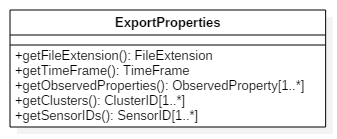
\includegraphics[width=0.4\linewidth]{images/export/classes/ExportProperties}
\end{figure}
\subsubsection{Declaration}{
\begin{lstlisting}[frame=none]
public class ExportProperties
 extends java.lang.Object\end{lstlisting}
\subsubsection{Constructor summary}{
\begin{verse}
\hyperlink{Export.ExportProperties()}{{\bf ExportProperties()}} Default constructor\\
\end{verse}
}
\subsubsection{Method summary}{
\begin{verse}
\hyperlink{Export.ExportProperties.getClusters()}{{\bf getClusters()}} Get the ClusterIDs that should be exported.\\
\hyperlink{Export.ExportProperties.getFileExtension()}{{\bf getFileExtension()}} Get the FileExtension for the Export File.\\
\hyperlink{Export.ExportProperties.getObservedProperties()}{{\bf getObservedProperties()}} Get the ObsorvedProperties that should be exported.\\
\hyperlink{Export.ExportProperties.getSensorIDs()}{{\bf getSensorIDs()}} Get the SensorIDs that should be exported.\\
\hyperlink{Export.ExportProperties.getTimeFrame()}{{\bf getTimeFrame()}} Get the TimeFrame of the Data that should be exported.\\
\end{verse}
}
\subsubsection{Constructors}{
\vskip -2em
\begin{itemize}
\item{
\index{ExportProperties()}
\hypertarget{Export.ExportProperties()}{{\bf  ExportProperties}\\}
\begin{lstlisting}[frame=none]
public ExportProperties()\end{lstlisting} %end signature
\begin{itemize}
\item{
{\bf  Description}

Default constructor
}
\end{itemize}
}%end item
\end{itemize}
}
\subsubsection{Methods}{
\vskip -2em
\begin{itemize}
\item{
\index{getClusters()}
\hypertarget{Export.ExportProperties.getClusters()}{{\bf  getClusters}\\}
\begin{lstlisting}[frame=none]
public java.util.Set getClusters()\end{lstlisting} %end signature
\begin{itemize}
\item{
{\bf  Description}

Get the ClusterIDs that should be exported. Always only exports a Groupd of Sensors or a Group of Clusters. The other Option is Empty.
}
\item{{\bf  Returns} --
The Clusters that should be taken in the Export.
}%end item
\end{itemize}
}%end item
\item{
\index{getFileExtension()}
\hypertarget{Export.ExportProperties.getFileExtension()}{{\bf  getFileExtension}\\}
\begin{lstlisting}[frame=none]
public FileExtension getFileExtension()\end{lstlisting} %end signature
\begin{itemize}
\item{
{\bf  Description}

Get the FileExtension for the Export File.
}
\item{{\bf  Returns} --
The FileExtension for the File to export.
}%end item
\end{itemize}
}%end item
\item{
\index{getObservedProperties()}
\hypertarget{Export.ExportProperties.getObservedProperties()}{{\bf  getObservedProperties}\\}
\begin{lstlisting}[frame=none]
public java.util.Set getObservedProperties()\end{lstlisting} %end signature
\begin{itemize}
\item{
{\bf  Description}

Get the ObsorvedProperties that should be exported.
}
\item{{\bf  Returns} --
The ObservedProperties that should be used for the export.
}%end item
\end{itemize}
}%end item
\item{
\index{getSensorIDs()}
\hypertarget{Export.ExportProperties.getSensorIDs()}{{\bf  getSensorIDs}\\}
\begin{lstlisting}[frame=none]
public java.util.Set getSensorIDs()\end{lstlisting} %end signature
\begin{itemize}
\item{
{\bf  Description}

Get the SensorIDs that should be exported. Always only exports a Groupd of Sensors or a Group of Clusters. The other Option is Empty.
}
\item{{\bf  Returns} --
The SensorIDs of the Data that should be exported.
}%end item
\end{itemize}
}%end item
\item{
\index{getTimeFrame()}
\hypertarget{Export.ExportProperties.getTimeFrame()}{{\bf  getTimeFrame}\\}
\begin{lstlisting}[frame=none]
public TimeFrame getTimeFrame()\end{lstlisting} %end signature
\begin{itemize}
\item{
{\bf  Description}

Get the TimeFrame of the Data that should be exported.
}
\item{{\bf  Returns} --
The TimeFrame of the Data to be exported.
}%end item
\end{itemize}
}%end item
\end{itemize}
}
}
\newpage
\subsection{\label{Export.ExportStreamGenerator}Class ExportStreamGenerator}{
\hypertarget{Export.ExportStreamGenerator}{}\vskip .1in
Generates a Stream for the Export by asking for one at the PaVoS Core and Subscribing to it.\vskip .1in
\begin{figure}[!hbp]
	\centering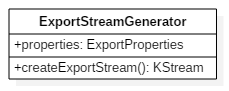
\includegraphics[width=0.4\linewidth]{images/export/classes/ExportStreamGenerator}
\end{figure}
\subsubsection{Declaration}{
\begin{lstlisting}[frame=none]
public class ExportStreamGenerator
 extends java.lang.Object\end{lstlisting}
\subsubsection{Field summary}{
\begin{verse}
\hyperlink{Export.ExportStreamGenerator.properties}{{\bf properties}} Contains the Properties of an Export Request.\\
\end{verse}
}
\subsubsection{Constructor summary}{
\begin{verse}
\hyperlink{Export.ExportStreamGenerator()}{{\bf ExportStreamGenerator()}} Default constructor\\
\end{verse}
}
\subsubsection{Method summary}{
\begin{verse}
\hyperlink{Export.ExportStreamGenerator.createExportStream()}{{\bf createExportStream()}} Asks for a KafkaStream and subscribes to it.\\
\end{verse}
}
\subsubsection{Fields}{
\begin{itemize}
\item{
\index{properties}
\label{Export.ExportStreamGenerator.properties}\hypertarget{Export.ExportStreamGenerator.properties}{\texttt{public ExportProperties\ {\bf  properties}}
}
\begin{itemize}
\item{\vskip -.9ex
Contains the Properties of an Export Request.}
\end{itemize}
}
\end{itemize}
}
\subsubsection{Constructors}{
\vskip -2em
\begin{itemize}
\item{
\index{ExportStreamGenerator()}
\hypertarget{Export.ExportStreamGenerator()}{{\bf  ExportStreamGenerator}\\}
\begin{lstlisting}[frame=none]
public ExportStreamGenerator()\end{lstlisting} %end signature
\begin{itemize}
\item{
{\bf  Description}

Default constructor
}
\end{itemize}
}%end item
\end{itemize}
}
\subsubsection{Methods}{
\vskip -2em
\begin{itemize}
\item{
\index{createExportStream()}
\hypertarget{Export.ExportStreamGenerator.createExportStream()}{{\bf  createExportStream}\\}
\begin{lstlisting}[frame=none]
public KStream createExportStream()\end{lstlisting} %end signature
\begin{itemize}
\item{
{\bf  Description}

Asks for a KafkaStream and subscribes to it. Then gives it through to the needed part for the export.
}
\item{{\bf  Returns} --
Is a KStream of the Data that should be exported.
}%end item
\end{itemize}
}%end item
\end{itemize}
}
}
\subsection{\label{Export.FileExporter}Class FileExporter}{
\hypertarget{Export.FileExporter}{}\vskip .1in
Exporter of Data from Kafka to a File.\vskip .1in
\begin{figure}[!hbp]
	\centering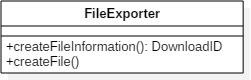
\includegraphics[width=0.4\linewidth]{images/export/classes/FileExporter}
\end{figure}
\subsubsection{Declaration}{
\begin{lstlisting}[frame=none]
public class FileExporter
 extends Export.AbstractExporter\end{lstlisting}
\subsubsection{Constructor summary}{
\begin{verse}
\hyperlink{Export.FileExporter()}{{\bf FileExporter()}} Default constructor\\
\end{verse}
}
\subsubsection{Method summary}{
\begin{verse}
\hyperlink{Export.FileExporter.createFile()}{{\bf createFile()}} Generates the File with the desired Data.\\
\hyperlink{Export.FileExporter.createFileInformation()}{{\bf createFileInformation()}} Creates Information for that Export.\\
\end{verse}
}
\subsubsection{Constructors}{
\vskip -2em
\begin{itemize}
\item{
\index{FileExporter()}
\hypertarget{Export.FileExporter()}{{\bf  FileExporter}\\}
\begin{lstlisting}[frame=none]
public FileExporter()\end{lstlisting} %end signature
\begin{itemize}
\item{
{\bf  Description}

Default constructor
}
\end{itemize}
}%end item
\end{itemize}
}
\subsubsection{Methods}{
\vskip -2em
\begin{itemize}
\item{
\index{createFile()}
\hypertarget{Export.FileExporter.createFile()}{{\bf  createFile}\\}
\begin{lstlisting}[frame=none]
public void createFile()\end{lstlisting} %end signature
\begin{itemize}
\item{
{\bf  Description}

Generates the File with the desired Data.
}
\end{itemize}
}%end item
\item{
\index{createFileInformation()}
\hypertarget{Export.FileExporter.createFileInformation()}{{\bf  createFileInformation}\\}
\begin{lstlisting}[frame=none]
public DownloadID createFileInformation()\end{lstlisting} %end signature
\begin{itemize}
\item{
{\bf  Description}

Creates Information for that Export. These Information will be used to identifie a File for the WebGUI, that gets the created DownloadID.
}
\item{{\bf  Returns} --
Is the DownloadID for the started Export.
}%end item
\end{itemize}
}%end item
\end{itemize}
}
\subsubsection{Members inherited from class AbstractExporter }{
\texttt{Export.AbstractExporter} {\small
\refdefined{Export.AbstractExporter}}
{\small

\vskip -2em
\begin{itemize}
\item{\vskip -1.5ex
\texttt{public void {\bf  createFile}()
}%end signature
}%end item
\item{\vskip -1.5ex
\texttt{public DownloadID {\bf  createFileInformation}()
}%end signature
}%end item
\item{\vskip -1.5ex
\texttt{public {\bf  properties}}%end signature
}%end item
\end{itemize}
}
}
\subsection{\label{Export.FileExtension}Class FileExtension}{
\hypertarget{Export.FileExtension}{}\vskip .1in
Represents the FileExtension of a File. Is used to match the right FileFormat for an export or import.\vskip .1in
\begin{figure}[!hbp]
	\centering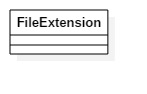
\includegraphics[width=0.2\linewidth]{images/export/classes/FileExtension}
\end{figure}
\subsubsection{Declaration}{
\begin{lstlisting}[frame=none]
public class FileExtension
 extends java.lang.Object\end{lstlisting}
\subsubsection{Constructor summary}{
\begin{verse}
\hyperlink{Export.FileExtension()}{{\bf FileExtension()}} Default constructor\\
\end{verse}
}
\subsubsection{Constructors}{
\vskip -2em
\begin{itemize}
\item{
\index{FileExtension()}
\hypertarget{Export.FileExtension()}{{\bf  FileExtension}\\}
\begin{lstlisting}[frame=none]
public FileExtension()\end{lstlisting} %end signature
\begin{itemize}
\item{
{\bf  Description}

Default constructor
}
\end{itemize}
}%end item
\end{itemize}
}
}
\subsection{\label{Export.FileType}Class FileType}{
\hypertarget{Export.FileType}{}\vskip .1in
Is used to store a FileExtension information and give the right FileWriter for this FileExtension.\vskip .1in
\begin{figure}[!hbp]
	\centering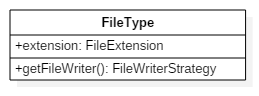
\includegraphics[width=0.4\linewidth]{images/export/classes/FileType}
\end{figure}
\subsubsection{Declaration}{
\begin{lstlisting}[frame=none]
public class FileType
 extends java.lang.Object\end{lstlisting}
\subsubsection{Field summary}{
\begin{verse}
\hyperlink{Export.FileType.extension}{{\bf extension}} The FileExtension is defining the FileType.\\
\end{verse}
}
\subsubsection{Constructor summary}{
\begin{verse}
\hyperlink{Export.FileType()}{{\bf FileType()}} Default constructor\\
\end{verse}
}
\subsubsection{Method summary}{
\begin{verse}
\hyperlink{Export.FileType.getFileWriter()}{{\bf getFileWriter()}} Gives an instance of the implemented FileWriter that is associated with this FileType, thus this FileExtension.\\
\end{verse}
}
\subsubsection{Fields}{
\begin{itemize}
\item{
\index{extension}
\label{Export.FileType.extension}\hypertarget{Export.FileType.extension}{\texttt{public FileExtension\ {\bf  extension}}
}
\begin{itemize}
\item{\vskip -.9ex
The FileExtension is defining the FileType.}
\end{itemize}
}
\end{itemize}
}
\subsubsection{Constructors}{
\vskip -2em
\begin{itemize}
\item{
\index{FileType()}
\hypertarget{Export.FileType()}{{\bf  FileType}\\}
\begin{lstlisting}[frame=none]
public FileType()\end{lstlisting} %end signature
\begin{itemize}
\item{
{\bf  Description}

Default constructor
}
\end{itemize}
}%end item
\end{itemize}
}
\subsubsection{Methods}{
\vskip -2em
\begin{itemize}
\item{
\index{getFileWriter()}
\hypertarget{Export.FileType.getFileWriter()}{{\bf  getFileWriter}\\}
\begin{lstlisting}[frame=none]
public FileWriterStrategy getFileWriter()\end{lstlisting} %end signature
\begin{itemize}
\item{
{\bf  Description}

Gives an instance of the implemented FileWriter that is associated with this FileType, thus this FileExtension. To do so it uses the static method getFileWriterForFileExtension from the FileTypesUtility class.
}
\item{{\bf  Returns} --
Is a new instance of an implementation of a FilWriterStrategy.
}%end item
\end{itemize}
}%end item
\end{itemize}
}
}
\subsection{\label{Export.FileTypesUtility}Class FileTypesUtility}{
\hypertarget{Export.FileTypesUtility}{}\vskip .1in
Utility class that provides static methods to get all supported FileExtensions and one to get a new Instance of the FileWriter associated with a given FileExtension. If a new FileWriter is added to PaVoS, this class needs some changed to be able to return the new FileWriter.\vskip .1in
\begin{figure}[!hbp]
	\centering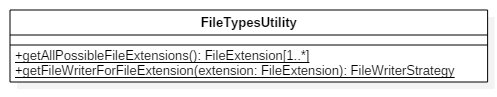
\includegraphics[width=0.6\linewidth]{images/export/classes/FileTypesUtility}
\end{figure}
\subsubsection{Declaration}{
\begin{lstlisting}[frame=none]
public class FileTypesUtility
 extends java.lang.Object\end{lstlisting}
\subsubsection{Constructor summary}{
\begin{verse}
\hyperlink{Export.FileTypesUtility()}{{\bf FileTypesUtility()}} Default constructor\\
\end{verse}
}
\subsubsection{Method summary}{
\begin{verse}
\hyperlink{Export.FileTypesUtility.getAllPossibleFileExtensions()}{{\bf getAllPossibleFileExtensions()}} Gives all supported FileExtensions in an ArrayList.\\
\hyperlink{Export.FileTypesUtility.getFileWriterForFileExtension(Export.FileExtension)}{{\bf getFileWriterForFileExtension(FileExtension)}} Gives a new Instance of the FileWriter associated witha given FileExtension.\\
\end{verse}
}
\subsubsection{Constructors}{
\vskip -2em
\begin{itemize}
\item{
\index{FileTypesUtility()}
\hypertarget{Export.FileTypesUtility()}{{\bf  FileTypesUtility}\\}
\begin{lstlisting}[frame=none]
public FileTypesUtility()\end{lstlisting} %end signature
\begin{itemize}
\item{
{\bf  Description}

Default constructor
}
\end{itemize}
}%end item
\end{itemize}
}
\subsubsection{Methods}{
\vskip -2em
\begin{itemize}
\item{
\index{getAllPossibleFileExtensions()}
\hypertarget{Export.FileTypesUtility.getAllPossibleFileExtensions()}{{\bf  getAllPossibleFileExtensions}\\}
\begin{lstlisting}[frame=none]
public static java.util.Set getAllPossibleFileExtensions()\end{lstlisting} %end signature
\begin{itemize}
\item{
{\bf  Description}

Gives all supported FileExtensions in an ArrayList.
}
\item{{\bf  Returns} --
Is an Array of the possible FileExtensions for an Export.
}%end item
\end{itemize}
}%end item
\item{
\index{getFileWriterForFileExtension(FileExtension)}
\hypertarget{Export.FileTypesUtility.getFileWriterForFileExtension(Export.FileExtension)}{{\bf  getFileWriterForFileExtension}\\}
\begin{lstlisting}[frame=none]
public static FileWriterStrategy getFileWriterForFileExtension(FileExtension extension)\end{lstlisting} %end signature
\begin{itemize}
\item{
{\bf  Description}

Gives a new Instance of the FileWriter associated witha given FileExtension.
}
\item{
{\bf  Parameters}
  \begin{itemize}
   \item{
\texttt{extension} -- Is the FileExtension for which a new instance of an Implementation of the FileWriterStrategy is wanted.}
  \end{itemize}
}%end item
\item{{\bf  Returns} --
Is the instance of the implementation of a FileWriterStrategy.
}%end item
\end{itemize}
}%end item
\end{itemize}
}
}
\newpage
\subsection{\label{Export.NetCDFWriterStrategy}Class NetCDFWriterStrategy}{
\hypertarget{Export.NetCDFWriterStrategy}{}\vskip .1in
Implementation of the FileWriterStrategy interface for NetCDF files.\vskip .1in
\begin{figure}[!hbp]
	\centering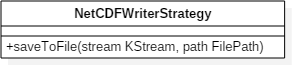
\includegraphics[width=0.5\linewidth]{images/export/classes/NetCDFWriterStrategy}
\end{figure}
\subsubsection{Declaration}{
\begin{lstlisting}[frame=none]
public class NetCDFWriterStrategy
 extends java.lang.Object implements FileWriterStrategy\end{lstlisting}
\subsubsection{Constructor summary}{
\begin{verse}
\hyperlink{Export.NetCDFWriterStrategy()}{{\bf NetCDFWriterStrategy()}} Default constructor\\
\end{verse}
}
\subsubsection{Method summary}{
\begin{verse}
\hyperlink{Export.NetCDFWriterStrategy.saveToFile(KStream, FilePath)}{{\bf saveToFile(KStream, FilePath)}} Creates a File as specified by the FilePath and saves the Data from the provided KafkaStream into it.\\
\hyperlink{Export.NetCDFWriterStrategy.saveToFile(KStream, FilePath)}{{\bf saveToFile(KStream, FilePath)}} Creates a File as specified by the FilePath and saves the Data from the provided KafkaStream into it.\\
\end{verse}
}
\subsubsection{Constructors}{
\vskip -2em
\begin{itemize}
\item{
\index{NetCDFWriterStrategy()}
\hypertarget{Export.NetCDFWriterStrategy()}{{\bf  NetCDFWriterStrategy}\\}
\begin{lstlisting}[frame=none]
public NetCDFWriterStrategy()\end{lstlisting} %end signature
\begin{itemize}
\item{
{\bf  Description}

Default constructor
}
\end{itemize}
}%end item
\end{itemize}
}
\subsubsection{Methods}{
\vskip -2em
\begin{itemize}
\item{
\index{saveToFile(KStream, FilePath)}
\hypertarget{Export.NetCDFWriterStrategy.saveToFile(KStream, FilePath)}{{\bf  saveToFile}\\}
\begin{lstlisting}[frame=none]
public void saveToFile(KStream stream,FilePath path)\end{lstlisting} %end signature
\begin{itemize}
\item{
{\bf  Description}

Creates a File as specified by the FilePath and saves the Data from the provided KafkaStream into it.
}
\item{
{\bf  Parameters}
  \begin{itemize}
   \item{
\texttt{stream} -- is the KStream, that should be exported to a File.}
   \item{
\texttt{path} -- Is the FilePath, where the new File should be created.}
  \end{itemize}
}%end item
\end{itemize}
}%end item
\item{
\index{saveToFile(KStream, FilePath)}
\hypertarget{Export.NetCDFWriterStrategy.saveToFile(KStream, FilePath)}{{\bf  saveToFile}\\}
\begin{lstlisting}[frame=none]
public void saveToFile(KStream stream,FilePath path)\end{lstlisting} %end signature
\begin{itemize}
\item{
{\bf  Description}

Creates a File as specified by the FilePath and saves the Data from the provided KafkaStream into it.
}
\item{
{\bf  Parameters}
  \begin{itemize}
   \item{
\texttt{stream} -- is the KStream, that should be exported to a File.}
   \item{
\texttt{path} -- Is the FilePath, where the new File should be created.}
  \end{itemize}
}%end item
\end{itemize}
}%end item
\end{itemize}
}
}
}
\newpage
\section{Package Download}{
\label{Download}\hypertarget{Download}{}
\hskip -.05in
\hbox to \hsize{\textit{ Package Contents\hfil Page}}
\vskip .13in
\hbox{{\bf  Classes}}
\entityintro{AlterableDownloadState}{Download.AlterableDownloadState}{Verifies for the State of a Download.}
\entityintro{DownloadID}{Download.DownloadID}{Is an Identifier for a specific Download, so that the right file can be fount for a requeststed Download.}
\entityintro{DownloadState}{Download.DownloadState}{Verifies for the State of a Download.}
\vskip .1in
\vskip .1in
\subsection{\label{Download.AlterableDownloadState}Class AlterableDownloadState}{
\hypertarget{Download.AlterableDownloadState}{}\vskip .1in
Verifies for the State of a Download. Can also change it.\vskip .1in
\begin{figure}[!hbp]
	\centering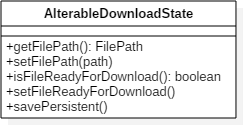
\includegraphics[width=0.4\linewidth]{images/export/classes/AlterableDownloadState}
\end{figure}
\subsubsection{Declaration}{
\begin{lstlisting}[frame=none]
public class AlterableDownloadState
 extends Download.DownloadState\end{lstlisting}
\subsubsection{Constructor summary}{
\begin{verse}
\hyperlink{Download.AlterableDownloadState()}{{\bf AlterableDownloadState()}} Default constructor\\
\end{verse}
}
\subsubsection{Method summary}{
\begin{verse}
\hyperlink{Download.AlterableDownloadState.getFilePath()}{{\bf getFilePath()}} Gives the FilePath associated with this DownloadID.\\
\hyperlink{Download.AlterableDownloadState.isFileReadyForDownload()}{{\bf isFileReadyForDownload()}} Checks if a File is Ready to be downloaded.\\
\hyperlink{Download.AlterableDownloadState.savePersistent()}{{\bf savePersistent()}} Save the changed Data persistently.\\
\hyperlink{Download.AlterableDownloadState.setFilePath(void)}{{\bf setFilePath(void)}} Defines the FilePath for the DownloadID.\\
\hyperlink{Download.AlterableDownloadState.setFileReadyForDownload()}{{\bf setFileReadyForDownload()}} Validate, that the File is ready to be downloaded.\\
\end{verse}
}
\subsubsection{Constructors}{
\vskip -2em
\begin{itemize}
\item{
\index{AlterableDownloadState()}
\hypertarget{Download.AlterableDownloadState()}{{\bf  AlterableDownloadState}\\}
\begin{lstlisting}[frame=none]
public AlterableDownloadState()\end{lstlisting} %end signature
\begin{itemize}
\item{
{\bf  Description}

Default constructor
}
\end{itemize}
}%end item
\end{itemize}
}
\subsubsection{Methods}{
\vskip -2em
\begin{itemize}
\item{
\index{getFilePath()}
\hypertarget{Download.AlterableDownloadState.getFilePath()}{{\bf  getFilePath}\\}
\begin{lstlisting}[frame=none]
public FilePath getFilePath()\end{lstlisting} %end signature
\begin{itemize}
\item{
{\bf  Description}

Gives the FilePath associated with this DownloadID.
}
\item{{\bf  Returns} --
The FilePath of the File for the Download.
}%end item
\end{itemize}
}%end item
\item{
\index{isFileReadyForDownload()}
\hypertarget{Download.AlterableDownloadState.isFileReadyForDownload()}{{\bf  isFileReadyForDownload}\\}
\begin{lstlisting}[frame=none]
public boolean isFileReadyForDownload()\end{lstlisting} %end signature
\begin{itemize}
\item{
{\bf  Description}

Checks if a File is Ready to be downloaded.
}
\item{{\bf  Returns} --
A boolean whether the file is downloadable or not.
}%end item
\end{itemize}
}%end item
\item{
\index{savePersistent()}
\hypertarget{Download.AlterableDownloadState.savePersistent()}{{\bf  savePersistent}\\}
\begin{lstlisting}[frame=none]
public void savePersistent()\end{lstlisting} %end signature
\begin{itemize}
\item{
{\bf  Description}

Save the changed Data persistently.
}
\end{itemize}
}%end item
\item{
\index{setFilePath(void)}
\hypertarget{Download.AlterableDownloadState.setFilePath(void)}{{\bf  setFilePath}\\}
\begin{lstlisting}[frame=none]
public void setFilePath(void path)\end{lstlisting} %end signature
\begin{itemize}
\item{
{\bf  Description}

Defines the FilePath for the DownloadID.
}
\item{
{\bf  Parameters}
  \begin{itemize}
   \item{
\texttt{path} -- Is the FilePath to be set.}
  \end{itemize}
}%end item
\end{itemize}
}%end item
\item{
\index{setFileReadyForDownload()}
\hypertarget{Download.AlterableDownloadState.setFileReadyForDownload()}{{\bf  setFileReadyForDownload}\\}
\begin{lstlisting}[frame=none]
public void setFileReadyForDownload()\end{lstlisting} %end signature
\begin{itemize}
\item{
{\bf  Description}

Validate, that the File is ready to be downloaded.
}
\end{itemize}
}%end item
\end{itemize}
}
\subsubsection{Members inherited from class DownloadState }{
\texttt{Download.DownloadState} {\small
\refdefined{Download.DownloadState}}
{\small

\vskip -2em
\begin{itemize}
\item{\vskip -1.5ex
\texttt{public {\bf  downloadID}}%end signature
}%end item
\item{\vskip -1.5ex
\texttt{public FilePath {\bf  getFilePath}()
}%end signature
}%end item
\item{\vskip -1.5ex
\texttt{public boolean {\bf  isFileReadyForDownload}()
}%end signature
}%end item
\end{itemize}
}
}
\subsection{\label{Download.DownloadID}Class DownloadID}{
\hypertarget{Download.DownloadID}{}\vskip .1in
Is an Identifier for a specific Download, so that the right file can be fount for a requeststed Download.\vskip .1in
\begin{figure}[!hbp]
	\centering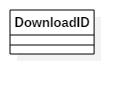
\includegraphics[width=0.2\linewidth]{images/export/classes/DownloadID}
\end{figure}
\subsubsection{Declaration}{
\begin{lstlisting}[frame=none]
public class DownloadID
 extends java.lang.Object\end{lstlisting}
\subsubsection{Constructor summary}{
\begin{verse}
\hyperlink{Download.DownloadID()}{{\bf DownloadID()}} Default constructor\\
\end{verse}
}
\subsubsection{Constructors}{
\vskip -2em
\begin{itemize}
\item{
\index{DownloadID()}
\hypertarget{Download.DownloadID()}{{\bf  DownloadID}\\}
\begin{lstlisting}[frame=none]
public DownloadID()\end{lstlisting} %end signature
\begin{itemize}
\item{
{\bf  Description}

Default constructor
}
\end{itemize}
}%end item
\end{itemize}
}
}
\subsection{\label{Download.DownloadState}Class DownloadState}{
\hypertarget{Download.DownloadState}{}\vskip .1in
Verifies for the State of a Download.\vskip .1in
\begin{figure}[!hbp]
	\centering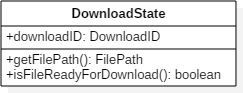
\includegraphics[width=0.4\linewidth]{images/export/classes/DownloadState}
\end{figure}
\subsubsection{Declaration}{
\begin{lstlisting}[frame=none]
public class DownloadState
 extends java.lang.Object\end{lstlisting}
\subsubsection{All known subclasses}{AlterableDownloadState\small{\refdefined{Download.AlterableDownloadState}}}
\subsubsection{Field summary}{
\begin{verse}
\hyperlink{Download.DownloadState.downloadID}{{\bf downloadID}} Is an Identifier for a specific Download.\\
\end{verse}
}
\subsubsection{Constructor summary}{
\begin{verse}
\hyperlink{Download.DownloadState()}{{\bf DownloadState()}} Default constructor\\
\end{verse}
}
\subsubsection{Method summary}{
\begin{verse}
\hyperlink{Download.DownloadState.getFilePath()}{{\bf getFilePath()}} Gives the FilePath associated with this DownloadID.\\
\hyperlink{Download.DownloadState.isFileReadyForDownload()}{{\bf isFileReadyForDownload()}} Checks if a File is Ready to be downloaded.\\
\end{verse}
}
\subsubsection{Fields}{
\begin{itemize}
\item{
\index{downloadID}
\label{Download.DownloadState.downloadID}\hypertarget{Download.DownloadState.downloadID}{\texttt{public DownloadID\ {\bf  downloadID}}
}
\begin{itemize}
\item{\vskip -.9ex
Is an Identifier for a specific Download.}
\end{itemize}
}
\end{itemize}
}
\subsubsection{Constructors}{
\vskip -2em
\begin{itemize}
\item{
\index{DownloadState()}
\hypertarget{Download.DownloadState()}{{\bf  DownloadState}\\}
\begin{lstlisting}[frame=none]
public DownloadState()\end{lstlisting} %end signature
\begin{itemize}
\item{
{\bf  Description}

Default constructor
}
\end{itemize}
}%end item
\end{itemize}
}
\subsubsection{Methods}{
\vskip -2em
\begin{itemize}
\item{
\index{getFilePath()}
\hypertarget{Download.DownloadState.getFilePath()}{{\bf  getFilePath}\\}
\begin{lstlisting}[frame=none]
public FilePath getFilePath()\end{lstlisting} %end signature
\begin{itemize}
\item{
{\bf  Description}

Gives the FilePath associated with this DownloadID.
}
\item{{\bf  Returns} --
The FilePath of the File for the Download.
}%end item
\end{itemize}
}%end item
\item{
\index{isFileReadyForDownload()}
\hypertarget{Download.DownloadState.isFileReadyForDownload()}{{\bf  isFileReadyForDownload}\\}
\begin{lstlisting}[frame=none]
public boolean isFileReadyForDownload()\end{lstlisting} %end signature
\begin{itemize}
\item{
{\bf  Description}

Checks if a File is Ready to be downloaded.
}
\item{{\bf  Returns} --
A boolean whether the file is downloadable or not.
}%end item
\end{itemize}
}%end item
\end{itemize}
}
}
}
\newpage
\section{Package ExportDownloadCommunication}{
\label{ExportDownloadCommunication}\hypertarget{ExportDownloadCommunication}{}
\hskip -.05in
\hbox to \hsize{\textit{ Package Contents\hfil Page}}
\vskip .13in
\hbox{{\bf  Classes}}
\entityintro{DownloadServlet}{ExportDownloadCommunication.DownloadServlet}{Servlet to let the WebGUI download a finished Export.}
\entityintro{ExportServlet}{ExportDownloadCommunication.ExportServlet}{HttpServlet to get a Dataexport request from the WebGUI.}
\entityintro{FileExtensionServlet}{ExportDownloadCommunication.FileExtensionServlet}{Servlet, to let the WebGUI ask for the available FileExtensions for the Export.}
\entityintro{HttpServlet}{ExportDownloadCommunication.HttpServlet}{Provides an abstract class to be subclassed to create an HTTP servlet suitable for a Web site.}
\entityintro{StatusServlet}{ExportDownloadCommunication.StatusServlet}{Servlet to let the WebGUI check if a Download is ready.}
\vskip .1in
\vskip .1in
\subsection{\label{ExportDownloadCommunication.DownloadServlet}Class DownloadServlet}{
\hypertarget{ExportDownloadCommunication.DownloadServlet}{}\vskip .1in
Servlet to let the WebGUI download a finished Export.\vskip .1in
\begin{figure}[!hbp]
	\centering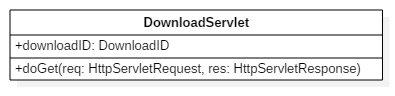
\includegraphics[width=0.7\linewidth]{images/export/classes/DownloadServlet}
\end{figure}
\subsubsection{Declaration}{
\begin{lstlisting}[frame=none]
public class DownloadServlet
 extends ExportDownloadCommunication.HttpServlet\end{lstlisting}
\subsubsection{Field summary}{
\begin{verse}
\hyperlink{ExportDownloadCommunication.DownloadServlet.downloadID}{{\bf downloadID}} Is an Identifier for a specific Download.\\
\end{verse}
}
\subsubsection{Constructor summary}{
\begin{verse}
\hyperlink{ExportDownloadCommunication.DownloadServlet()}{{\bf DownloadServlet()}} Default constructor\\
\end{verse}
}
\subsubsection{Method summary}{
\begin{verse}
\hyperlink{ExportDownloadCommunication.DownloadServlet.doGet(HttpServletRequest, HttpServletResponse)}{{\bf doGet(HttpServletRequest, HttpServletResponse)}} Handles a GET request by sending the desired File to the WebGUI.\\
\end{verse}
}
\subsubsection{Fields}{
\begin{itemize}
\item{
\index{downloadID}
\label{ExportDownloadCommunication.DownloadServlet.downloadID}\hypertarget{ExportDownloadCommunication.DownloadServlet.downloadID}{\texttt{public DownloadID\ {\bf  downloadID}}
}
\begin{itemize}
\item{\vskip -.9ex
Is an Identifier for a specific Download.}
\end{itemize}
}
\end{itemize}
}
\subsubsection{Constructors}{
\vskip -2em
\begin{itemize}
\item{
\index{DownloadServlet()}
\hypertarget{ExportDownloadCommunication.DownloadServlet()}{{\bf  DownloadServlet}\\}
\begin{lstlisting}[frame=none]
public DownloadServlet()\end{lstlisting} %end signature
\begin{itemize}
\item{
{\bf  Description}

Default constructor
}
\end{itemize}
}%end item
\end{itemize}
}
\subsubsection{Methods}{
\vskip -2em
\begin{itemize}
\item{
\index{doGet(HttpServletRequest, HttpServletResponse)}
\hypertarget{ExportDownloadCommunication.DownloadServlet.doGet(HttpServletRequest, HttpServletResponse)}{{\bf  doGet}\\}
\begin{lstlisting}[frame=none]
public void doGet(HttpServletRequest req,HttpServletResponse res)\end{lstlisting} %end signature
\begin{itemize}
\item{
{\bf  Description}

Handles a GET request by sending the desired File to the WebGUI.
}
\item{
{\bf  Parameters}
  \begin{itemize}
   \item{
\texttt{req} -- Is the HttpServletRequest.}
   \item{
\texttt{res} -- Is the HttpServletResponse.}
  \end{itemize}
}%end item
\end{itemize}
}%end item
\end{itemize}
}
\subsubsection{Members inherited from class HttpServlet }{
\texttt{ExportDownloadCommunication.HttpServlet} {\small
\refdefined{ExportDownloadCommunication.HttpServlet}}
{\small

\vskip -2em
\begin{itemize}
\item{\vskip -1.5ex
\texttt{public void {\bf  doGet}(\texttt{HttpServletRequest} {\bf  req},
\texttt{HttpServletResponse} {\bf  res})
}%end signature
}%end item
\end{itemize}
}
}
\newpage
\subsection{\label{ExportDownloadCommunication.ExportServlet}Class ExportServlet}{
\hypertarget{ExportDownloadCommunication.ExportServlet}{}\vskip .1in
HttpServlet to get a Dataexport request from the WebGUI.\vskip .1in
\begin{figure}[!hbp]
	\centering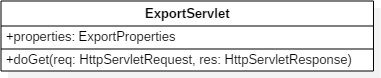
\includegraphics[width=0.7\linewidth]{images/export/classes/ExportServlet}
\end{figure}
\subsubsection{Declaration}{
\begin{lstlisting}[frame=none]
public class ExportServlet
 extends ExportDownloadCommunication.HttpServlet\end{lstlisting}
\subsubsection{Field summary}{
\begin{verse}
\hyperlink{ExportDownloadCommunication.ExportServlet.properties}{{\bf properties}} Contains the Properties of an Export Request.\\
\end{verse}
}
\subsubsection{Constructor summary}{
\begin{verse}
\hyperlink{ExportDownloadCommunication.ExportServlet()}{{\bf ExportServlet()}} Default constructor\\
\end{verse}
}
\subsubsection{Method summary}{
\begin{verse}
\hyperlink{ExportDownloadCommunication.ExportServlet.doGet(HttpServletRequest, HttpServletResponse)}{{\bf doGet(HttpServletRequest, HttpServletResponse)}} Handles a GET request by starting the export of the desired Data.\\
\end{verse}
}
\subsubsection{Fields}{
\begin{itemize}
\item{
\index{properties}
\label{ExportDownloadCommunication.ExportServlet.properties}\hypertarget{ExportDownloadCommunication.ExportServlet.properties}{\texttt{public ExportProperties\ {\bf  properties}}
}
\begin{itemize}
\item{\vskip -.9ex
Contains the Properties of an Export Request.}
\end{itemize}
}
\end{itemize}
}
\subsubsection{Constructors}{
\vskip -2em
\begin{itemize}
\item{
\index{ExportServlet()}
\hypertarget{ExportDownloadCommunication.ExportServlet()}{{\bf  ExportServlet}\\}
\begin{lstlisting}[frame=none]
public ExportServlet()\end{lstlisting} %end signature
\begin{itemize}
\item{
{\bf  Description}

Default constructor
}
\end{itemize}
}%end item
\end{itemize}
}
\subsubsection{Methods}{
\vskip -2em
\begin{itemize}
\item{
\index{doGet(HttpServletRequest, HttpServletResponse)}
\hypertarget{ExportDownloadCommunication.ExportServlet.doGet(HttpServletRequest, HttpServletResponse)}{{\bf  doGet}\\}
\begin{lstlisting}[frame=none]
public void doGet(HttpServletRequest req,HttpServletResponse res)\end{lstlisting} %end signature
\begin{itemize}
\item{
{\bf  Description}

Handles a GET request by starting the export of the desired Data. At the same time a DownloadID is sent back to the WebGUI, so that it can check for the File.
}
\item{
{\bf  Parameters}
  \begin{itemize}
   \item{
\texttt{req} -- Is the HttpServletRequest.}
   \item{
\texttt{res} -- Is the HttpServletResponse.}
  \end{itemize}
}%end item
\end{itemize}
}%end item
\end{itemize}
}
\subsubsection{Members inherited from class HttpServlet }{
\texttt{ExportDownloadCommunication.HttpServlet} {\small
\refdefined{ExportDownloadCommunication.HttpServlet}}
{\small

\vskip -2em
\begin{itemize}
\item{\vskip -1.5ex
\texttt{public void {\bf  doGet}(\texttt{HttpServletRequest} {\bf  req},
\texttt{HttpServletResponse} {\bf  res})
}%end signature
}%end item
\end{itemize}
}
}
\subsection{\label{ExportDownloadCommunication.FileExtensionServlet}Class FileExtensionServlet}{
\hypertarget{ExportDownloadCommunication.FileExtensionServlet}{}\vskip .1in
Servlet, to let the WebGUI ask for the available FileExtensions for the Export.\vskip .1in
\begin{figure}[!hbp]
	\centering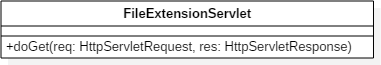
\includegraphics[width=0.7\linewidth]{images/export/classes/FileExtensionServlet}
\end{figure}
\subsubsection{Declaration}{
\begin{lstlisting}[frame=none]
public class FileExtensionServlet
 extends ExportDownloadCommunication.HttpServlet\end{lstlisting}
\subsubsection{Constructor summary}{
\begin{verse}
\hyperlink{ExportDownloadCommunication.FileExtensionServlet()}{{\bf FileExtensionServlet()}} Default constructor\\
\end{verse}
}
\subsubsection{Method summary}{
\begin{verse}
\hyperlink{ExportDownloadCommunication.FileExtensionServlet.doGet(HttpServletRequest, HttpServletResponse)}{{\bf doGet(HttpServletRequest, HttpServletResponse)}} Handles a GET request by sending Information about the available FileExtensions.\\
\end{verse}
}
\subsubsection{Constructors}{
\vskip -2em
\begin{itemize}
\item{
\index{FileExtensionServlet()}
\hypertarget{ExportDownloadCommunication.FileExtensionServlet()}{{\bf  FileExtensionServlet}\\}
\begin{lstlisting}[frame=none]
public FileExtensionServlet()\end{lstlisting} %end signature
\begin{itemize}
\item{
{\bf  Description}

Default constructor
}
\end{itemize}
}%end item
\end{itemize}
}
\subsubsection{Methods}{
\vskip -2em
\begin{itemize}
\item{
\index{doGet(HttpServletRequest, HttpServletResponse)}
\hypertarget{ExportDownloadCommunication.FileExtensionServlet.doGet(HttpServletRequest, HttpServletResponse)}{{\bf  doGet}\\}
\begin{lstlisting}[frame=none]
public void doGet(HttpServletRequest req,HttpServletResponse res)\end{lstlisting} %end signature
\begin{itemize}
\item{
{\bf  Description}

Handles a GET request by sending Information about the available FileExtensions.
}
\item{
{\bf  Parameters}
  \begin{itemize}
   \item{
\texttt{req} -- Is the HttpServletRequest.}
   \item{
\texttt{res} -- Is the HttpServletResponse.}
  \end{itemize}
}%end item
\end{itemize}
}%end item
\end{itemize}
}
\subsubsection{Members inherited from class HttpServlet }{
\texttt{ExportDownloadCommunication.HttpServlet} {\small
\refdefined{ExportDownloadCommunication.HttpServlet}}
{\small

\vskip -2em
\begin{itemize}
\item{\vskip -1.5ex
\texttt{public void {\bf  doGet}(\texttt{HttpServletRequest} {\bf  req},
\texttt{HttpServletResponse} {\bf  res})
}%end signature
}%end item
\end{itemize}
}
}
\subsection{\label{ExportDownloadCommunication.HttpServlet}Class HttpServlet}{
\hypertarget{ExportDownloadCommunication.HttpServlet}{}\vskip .1in
Provides an abstract class to be subclassed to create an HTTP servlet suitable for a Web site. (javax.servlet.http.HttpServlet)\vskip .1in
\begin{figure}[!hbp]
	\centering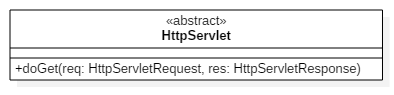
\includegraphics[width=0.7\linewidth]{images/export/classes/HttpServlet}
\end{figure}
\subsubsection{Declaration}{
\begin{lstlisting}[frame=none]
public class HttpServlet
 extends java.lang.Object\end{lstlisting}
\subsubsection{All known subclasses}{StatusServlet\small{\refdefined{ExportDownloadCommunication.StatusServlet}}, FileExtensionServlet\small{\refdefined{ExportDownloadCommunication.FileExtensionServlet}}, ExportServlet\small{\refdefined{ExportDownloadCommunication.ExportServlet}}, DownloadServlet\small{\refdefined{ExportDownloadCommunication.DownloadServlet}}}
\subsubsection{Constructor summary}{
\begin{verse}
\hyperlink{ExportDownloadCommunication.HttpServlet()}{{\bf HttpServlet()}} Default constructor\\
\end{verse}
}
\subsubsection{Method summary}{
\begin{verse}
\hyperlink{ExportDownloadCommunication.HttpServlet.doGet(HttpServletRequest, HttpServletResponse)}{{\bf doGet(HttpServletRequest, HttpServletResponse)}} Called by the server (via the service method) to allow a servlet to handle a GET request.\\
\end{verse}
}
\subsubsection{Constructors}{
\vskip -2em
\begin{itemize}
\item{
\index{HttpServlet()}
\hypertarget{ExportDownloadCommunication.HttpServlet()}{{\bf  HttpServlet}\\}
\begin{lstlisting}[frame=none]
public HttpServlet()\end{lstlisting} %end signature
\begin{itemize}
\item{
{\bf  Description}

Default constructor
}
\end{itemize}
}%end item
\end{itemize}
}
\subsubsection{Methods}{
\vskip -2em
\begin{itemize}
\item{
\index{doGet(HttpServletRequest, HttpServletResponse)}
\hypertarget{ExportDownloadCommunication.HttpServlet.doGet(HttpServletRequest, HttpServletResponse)}{{\bf  doGet}\\}
\begin{lstlisting}[frame=none]
public void doGet(HttpServletRequest req,HttpServletResponse res)\end{lstlisting} %end signature
\begin{itemize}
\item{
{\bf  Description}

Called by the server (via the service method) to allow a servlet to handle a GET request.
}
\item{
{\bf  Parameters}
  \begin{itemize}
   \item{
\texttt{req} -- Is the HttpServletRequest.}
   \item{
\texttt{res} -- Is the HttpServletResponse.}
  \end{itemize}
}%end item
\end{itemize}
}%end item
\end{itemize}
}
}
\newpage
\subsection{\label{ExportDownloadCommunication.StatusServlet}Class StatusServlet}{
\hypertarget{ExportDownloadCommunication.StatusServlet}{}\vskip .1in
Servlet to let the WebGUI check if a Download is ready.\vskip .1in
\begin{figure}[!hbp]
	\centering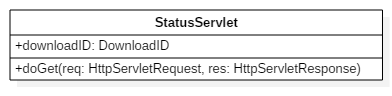
\includegraphics[width=0.7\linewidth]{images/export/classes/StatusServlet}
\end{figure}
\subsubsection{Declaration}{
\begin{lstlisting}[frame=none]
public class StatusServlet
 extends ExportDownloadCommunication.HttpServlet\end{lstlisting}
\subsubsection{Field summary}{
\begin{verse}
\hyperlink{ExportDownloadCommunication.StatusServlet.downloadID}{{\bf downloadID}} Is an Identifier for a specific Download.\\
\end{verse}
}
\subsubsection{Constructor summary}{
\begin{verse}
\hyperlink{ExportDownloadCommunication.StatusServlet()}{{\bf StatusServlet()}} Default constructor\\
\end{verse}
}
\subsubsection{Method summary}{
\begin{verse}
\hyperlink{ExportDownloadCommunication.StatusServlet.doGet(HttpServletRequest, HttpServletResponse)}{{\bf doGet(HttpServletRequest, HttpServletResponse)}} Handles a GET request by checking the availability of the desired download.\\
\end{verse}
}
\subsubsection{Fields}{
\begin{itemize}
\item{
\index{downloadID}
\label{ExportDownloadCommunication.StatusServlet.downloadID}\hypertarget{ExportDownloadCommunication.StatusServlet.downloadID}{\texttt{public DownloadID\ {\bf  downloadID}}
}
\begin{itemize}
\item{\vskip -.9ex
Is an Identifier for a specific Download.}
\end{itemize}
}
\end{itemize}
}
\subsubsection{Constructors}{
\vskip -2em
\begin{itemize}
\item{
\index{StatusServlet()}
\hypertarget{ExportDownloadCommunication.StatusServlet()}{{\bf  StatusServlet}\\}
\begin{lstlisting}[frame=none]
public StatusServlet()\end{lstlisting} %end signature
\begin{itemize}
\item{
{\bf  Description}

Default constructor
}
\end{itemize}
}%end item
\end{itemize}
}
\subsubsection{Methods}{
\vskip -2em
\begin{itemize}
\item{
\index{doGet(HttpServletRequest, HttpServletResponse)}
\hypertarget{ExportDownloadCommunication.StatusServlet.doGet(HttpServletRequest, HttpServletResponse)}{{\bf  doGet}\\}
\begin{lstlisting}[frame=none]
public void doGet(HttpServletRequest req,HttpServletResponse res)\end{lstlisting} %end signature
\begin{itemize}
\item{
{\bf  Description}

Handles a GET request by checking the availability of the desired download.
}
\item{
{\bf  Parameters}
  \begin{itemize}
   \item{
\texttt{req} -- Is the HttpServletRequest.}
   \item{
\texttt{res} -- Is the HttpServletResponse.}
  \end{itemize}
}%end item
\end{itemize}
}%end item
\end{itemize}
}
\subsubsection{Members inherited from class HttpServlet }{
\texttt{ExportDownloadCommunication.HttpServlet} {\small
\refdefined{ExportDownloadCommunication.HttpServlet}}
{\small

\vskip -2em
\begin{itemize}
\item{\vskip -1.5ex
\texttt{public void {\bf  doGet}(\texttt{HttpServletRequest} {\bf  req},
\texttt{HttpServletResponse} {\bf  res})
}%end signature
}%end item
\end{itemize}
}
}
}
